\subsection{Experiment Setup} \label{Experiment_Setup}
The experiment consisted of the AAC subsystem, with six sampling bags, and the CAC coiled tube subsystem. Shown in Figure {\ref{fig:3D_tubular_render}}, the AirCore was fitted into the CAC box, and the alternative sampling system with bags in the AAC box, together with the pneumatic system and the electronics placed inside the \emph{Brain}. The principal aim was to validate the AAC sampling method. To do so, it was necessary to sample during Descent Phase in order to compare the results with the ones obtained from the CAC. This was because the CAC collected its air sample passively by pressure differentials in the descent. Flight speeds mentioned in this section were obtained from the BEXUS manual as well as through analysis of past flights. Figure \ref{fig:block-diagram} shows a generic block diagram of the main subsystems interconnection.

\begin{figure}[H]
    \begin{align*}
        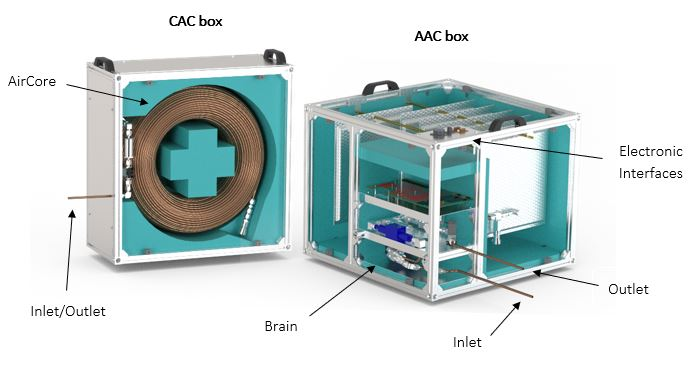
\includegraphics[width=1\linewidth]{4-experiment-design/img/Mechanical/tubular_render_labels.jpg}
    \end{align*}
    \caption{Physical Setup of the Experiment.}
    \label{fig:3D_tubular_render}
\end{figure}

\begin{figure}[H]
    \begin{align*}
        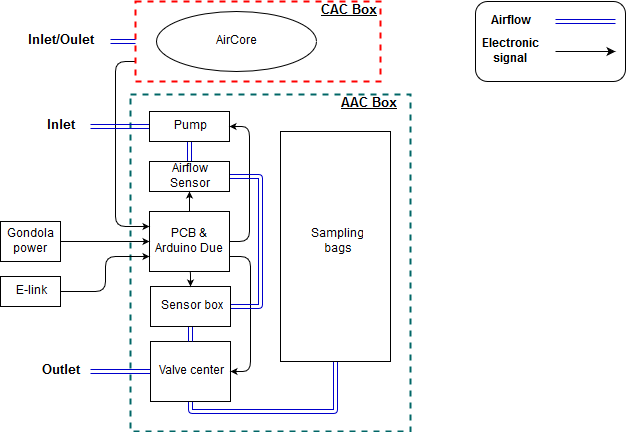
\includegraphics[width=1\linewidth]{4-experiment-design/img/Mechanical/Block-Diagram.png}
    \end{align*}
    \caption{Block Diagram of the Experiment.}
    \label{fig:block-diagram}
\end{figure}

The primary concern regarding the AAC air sampling subsystem occured after the cut-off while the gondola was tumbling and falling at an average speed of 50 m/s for approximately two minutes \cite{BexusManual}. This descent speed was too large in order to sample air at the desired vertical resolution, capped at 500 m. As such, sampling could only be done after the gondola had stabilized at a descent speed  of 8 m/s \cite{BexusManual}. The tumbling phase was vertically spanned for approximately 8 km. With a Float Phase altitude of approximately 27.3 km, sampling during the Descent Phase would have commenced at approximately 19 km in altitude. However, the primary region of interest in terms of sampling was in the stratosphere, particularly between 19 km and 27.3 km in altitude. This was why sampling was planned to also occur during the Ascent Phase. Out of the six sampling bags present in the payload, two were planned to be used during the Ascent Phase at 18 km and 21 km and four during the Descent Phase at 17.5 km, 16 km, 14 km and 12 km as seen in Table \ref{tab:minimum-volume}. Details regarding the sampling strategy can be found in Appendix \ref{sec:appH}.

%\begin{table}[H]
\centering
\begin{tabular}{|c|c|c|c|}
\hline
\multicolumn{1}{|l|}{} & \multicolumn{1}{l|}{\textbf{Sampling Altitudes}} & \multicolumn{1}{l|}{\textbf{Ambient Pressure}} & \multicolumn{1}{l|}{\textbf{Ambient Temperature}} \\ \hline
\multirow{2}{*}{\textbf{Ascent Phase}} & 18 km & 75.0 hPa & 216.7 K \\ \cline{2-4} 
 & 21 km & 46.8 hPa & 217.6 K \\ \hline
\multirow{4}{*}{\textbf{Descent Phase}} & 17.5 km & 81.2 hPa & 216.7 K \\ \cline{2-4} 
 & 16 km & 102.9 hPa & 216.7 K \\ \cline{2-4} 
 & 14 km & 141.0 hPa & 216.7 K \\ \cline{2-4} 
 & 12 km & 193.3 hPa & 216.7 K \\ \hline
\end{tabular}
\caption{Sampling Altitudes as well as the Corresponding Ambient Pressures and Temperatures According to the 1976 US Standard Atmosphere.}
\label{tab:sampling-altitudes}
\end{table}
The maximum pressure that the sampling bags could withstand had to be taken into account in order to avoid bursting. Decreasing pressure during the Ascent Phase would have posed a risk to sampling bags which already contained samples as the gas inside would expand which may cause the bag to burst. In order to avoid this, the sampling bags were not planned to be completely filled. Filling the sampling bags up to a maximum pressure of 2 psi/0.14 bar/140 hPa or alternatively filling the sampling bag up to 80\% of its capacity  was recommended by the manufacturers for the Multi-Layer Foil sampling bags that were used. Therefore, the expected maximum pressure inside the bags, that were filled during the Ascent Phase, would be 1.6 psi/0.11 bar/110 hPa. The inverse was also true for the Descent Phase where compression would occur. As such, the sampling bags had to be fully filled during the Descent Phase in order to ensure that enough samples were collected for analysis. During the Descent Phase, the expected maximum pressure inside the bags was expected to be 1.98 psi/0.13 bar/130 hPa. Past research had revealed that the selected sampling bags were able to withstand pressure difference of 310 hPa at 30 km of altitude, which was equivalent to 0.31 bar \cite{LISA}. Test 16 and 18, shown in Table \ref{tab:sampling-system-test} respective Table \ref{tab:pump-low-pressure-test},  were conducted in order to confirm the maximum allowable pressure for the bags.

The maximum operating pressure for the tubes, according to the manufacturers, was 2.2 psi/0.15 bar/150 hPa. The valve's leakage rate, given by the manufacturers, was 0.001 l/min.     


Due to the difference in pressure between sea level and sampling altitudes, the volume of the sample taken would have been considerably reduced when it reached sea level. This shrinking had to be taken into account as the minimum volume that had to be present in the sampling bag at sea level in order to obtain results with the Picarro analyzer. A minimum amount was required for the analyzer to detect concentrations of the targeted trace gases. This minimum amount was 0.18 L at sea level and it had to be specially considered for the samples taken at higher altitudes. The samples taken at lower altitudes were exposed to smaller changes in pressure, therefore their size was not critically reduced. Table \ref{tab:minimum-volume} shows the minimum volume of air that was needed to be sampled at different altitudes in order to assure the minimum air sample of 0.18L left at sea level. \\

This was the worst case scenario, and testing had shown that the higher the volume of the air sample left at sea level, the better the results. This was why the aimed volume of the samples, at sea level was at least 0.6L. 

%and the corresponding temperature and pressure conditions
 %pressure and temperature (288 K)  
% Depending on the sampling altitude,there is a minimum volume of air that needs to be sampled in order the sample volume left at sea level pressure is at least 0.18 L. A sample volume of 0.18 L corresponds to the minimum amount required for the Picarro analyzer to detect concentrations of the targeted trace gases. 

% Please add the following required packages to your document preamble:
% \usepackage{multirow}
\begin{table}[]
\centering
\begin{tabular}{|l|l|l|l|l|}
\hline
 & \textbf{\begin{tabular}[c]{@{}l@{}}Minimum \\ Sampling Volume\end{tabular}} & \textbf{\begin{tabular}[c]{@{}l@{}}Sampling \\ Altitudes\end{tabular}} & \textbf{\begin{tabular}[c]{@{}l@{}}Ambient \\ Pressure\end{tabular}} & \textbf{\begin{tabular}[c]{@{}l@{}}Ambient \\ Temperature\end{tabular}} \\ \hline
\multirow{2}{*}{\textbf{Ascent Phase}} & 1.8 L & 18 km & 75.0 hPa & 216.7 K \\ \cline{2-5} 
 & 2.4 L & 21 km & 46.8 hPa & 217.6 K \\ \hline
\multirow{4}{*}{\textbf{Descent Phase}} & 1.7 L & 17.5 km & 81.2 hPa & 216.7 K \\ \cline{2-5} 
 & 1.3 L & 16 km & 102.9 hPa & 216.7 K \\ \cline{2-5} 
 & 1.0 L & 14 km & 141.0 hPa & 216.7 K \\ \cline{2-5} 
 & 0.7 L & 12 km & 193.3 hPa & 216.7 K \\ \hline
\end{tabular}
\caption{Minimum Sampling Volume at Each Altitude to Obtain Enough Air to Perform a Proper Analysis (0.18 L at sea level), Appendix \ref{sec:appH}}
\label{tab:minimum-volume}
\end{table}


The AAC needed an air pump for sampling due to low ambient pressure at stratospheric altitudes. The air pump was also needed in order to assure the intake flow rate and obtain a good resolution. An air pump with an intake rate of at least 3 L/min was used to ensure that the vertical resolution of the sampling air remained under 500 m during the Ascent Phase's ascent speed of 5 m/s and the  Descent Phase's descent speed of 8 m/s. A flushing valve (see Figure \ref{pneumatic_system}, No.23) was used to flush the AAC system before each bag would have been filled and make sure that each bag would have been filled with fresh air from the corresponding altitude. This filling/flushing procedure was planned to occur twice, the first time during the Ascent Phase for the first two sampling bags and the second time during the Descent Phase for the remaining four sampling bags.

Shortly after the launch, the CAC valve was opened in order to allow the fill gas that was inside the tube to flush, while the AAC valves were closed until reaching the sampling altitude. Flushing of the CAC tube happened passively through the progressive decrease in air pressure during the balloon's Ascent Phase and it was emptied by the time it reached the Float Phase. Filling of the CAC tube also happened passively through the progressive increase in air pressure during the balloon's Descent Phase. The CAC valve was planned to  remain open at all time during the Ascent, Float, and Descent phases. Due to some problems, it was briefly closed and opened again for a few times without really compromising the results.  The valve should have been closed just before hitting the ground in order to preserve the sample. 

The ambient pressure was measured by three pressure sensors located outside the experiment box. Only one of them was necessary for AAC and CAC, but using three, redundancy was provided. To measure the pressure inside the bag that was currently being filled, one analogue static pressure sensor was connected to the pneumatic system. To measure the ambient temperature in the CAC, three sensors were allocated in the CAC box (in the Styrofoam). Temperature inside the coil was assumed to quickly adjust to the ambient temperature inside the CAC box, therefore there would not be differentiation in temperature between the air inside the tube and the air surrounding the tube. For the bags three more temperature sensors were placed in the bags' box (in the Styrofoam). To control the temperature for the pump and the valves in pneumatic subsystem, one temperature sensor was used for each of them. In total, there were three pressure sensors and eight temperature sensors. 

The sampling of the AAC was triggered by the pressure reading from the sensors outside the experiment box. When the required pressure was reached, as seen in Table \ref{tab:minimum-volume} the valve inside the manifold corresponding to the bag that was to be sampled, should have opened and the sampling should have started. The closing of the valve depended on two conditions and it was triggered when either one of the conditions was true. These conditions were: maximum sampling time or maximum pressure difference between inside/outside the bags. They were determined from past research \cite{LISA}. A first estimation of the maximum sampling time had already been made, from Test 18 shown in Table \ref{tab:pump-low-pressure-test}. Completed tests, such as Test 14 and Test 18, shown in Table \ref{tab:vacuum-test} respective Table \ref{tab:pump-low-pressure-test}, the maximum pressure condition had been determined and the maximum sampling times had been confirmed.

The CAC emptying as well as the AAC and CAC sampling sequence is represented in Figures \ref{fig:ascent} and \ref{fig:descent}. It should be kept in mind that the different pressures were what should have triggered the opening of the valves. 

\begin{figure}[H]
    \begin{align*}
        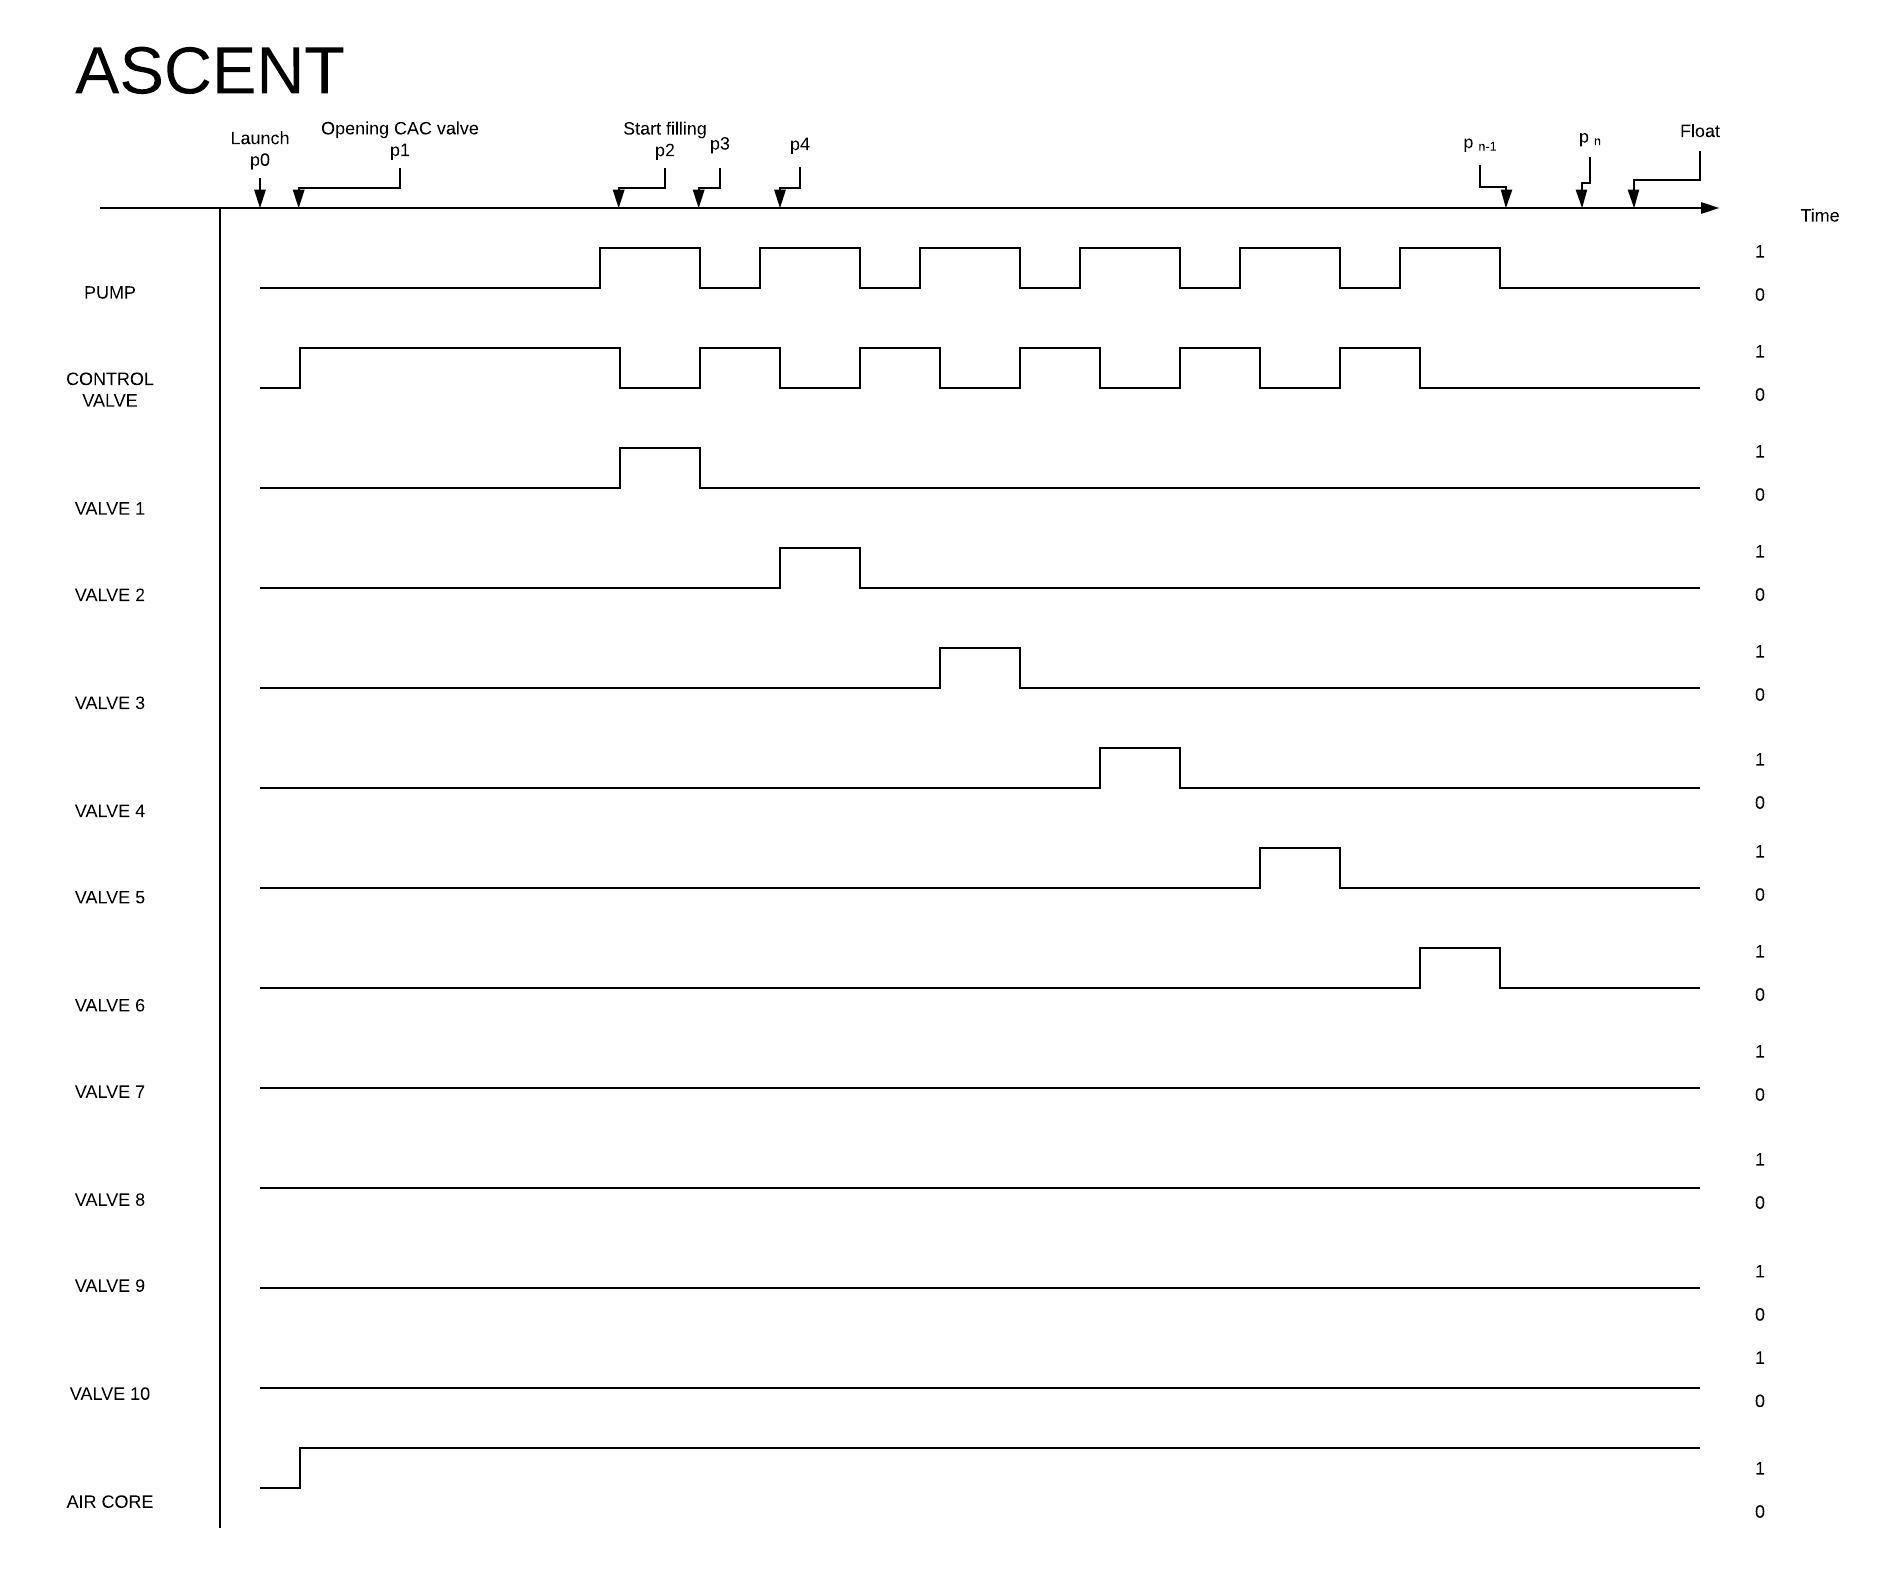
\includegraphics[width=1\linewidth]{4-experiment-design/img/ascent-phase.jpeg}
    \end{align*}
    \caption{The Emptying and Sampling Sequence-Ascent Phase.}
    \label{fig:ascent}
\end{figure}

\begin{figure}[H]
    \begin{align*}
        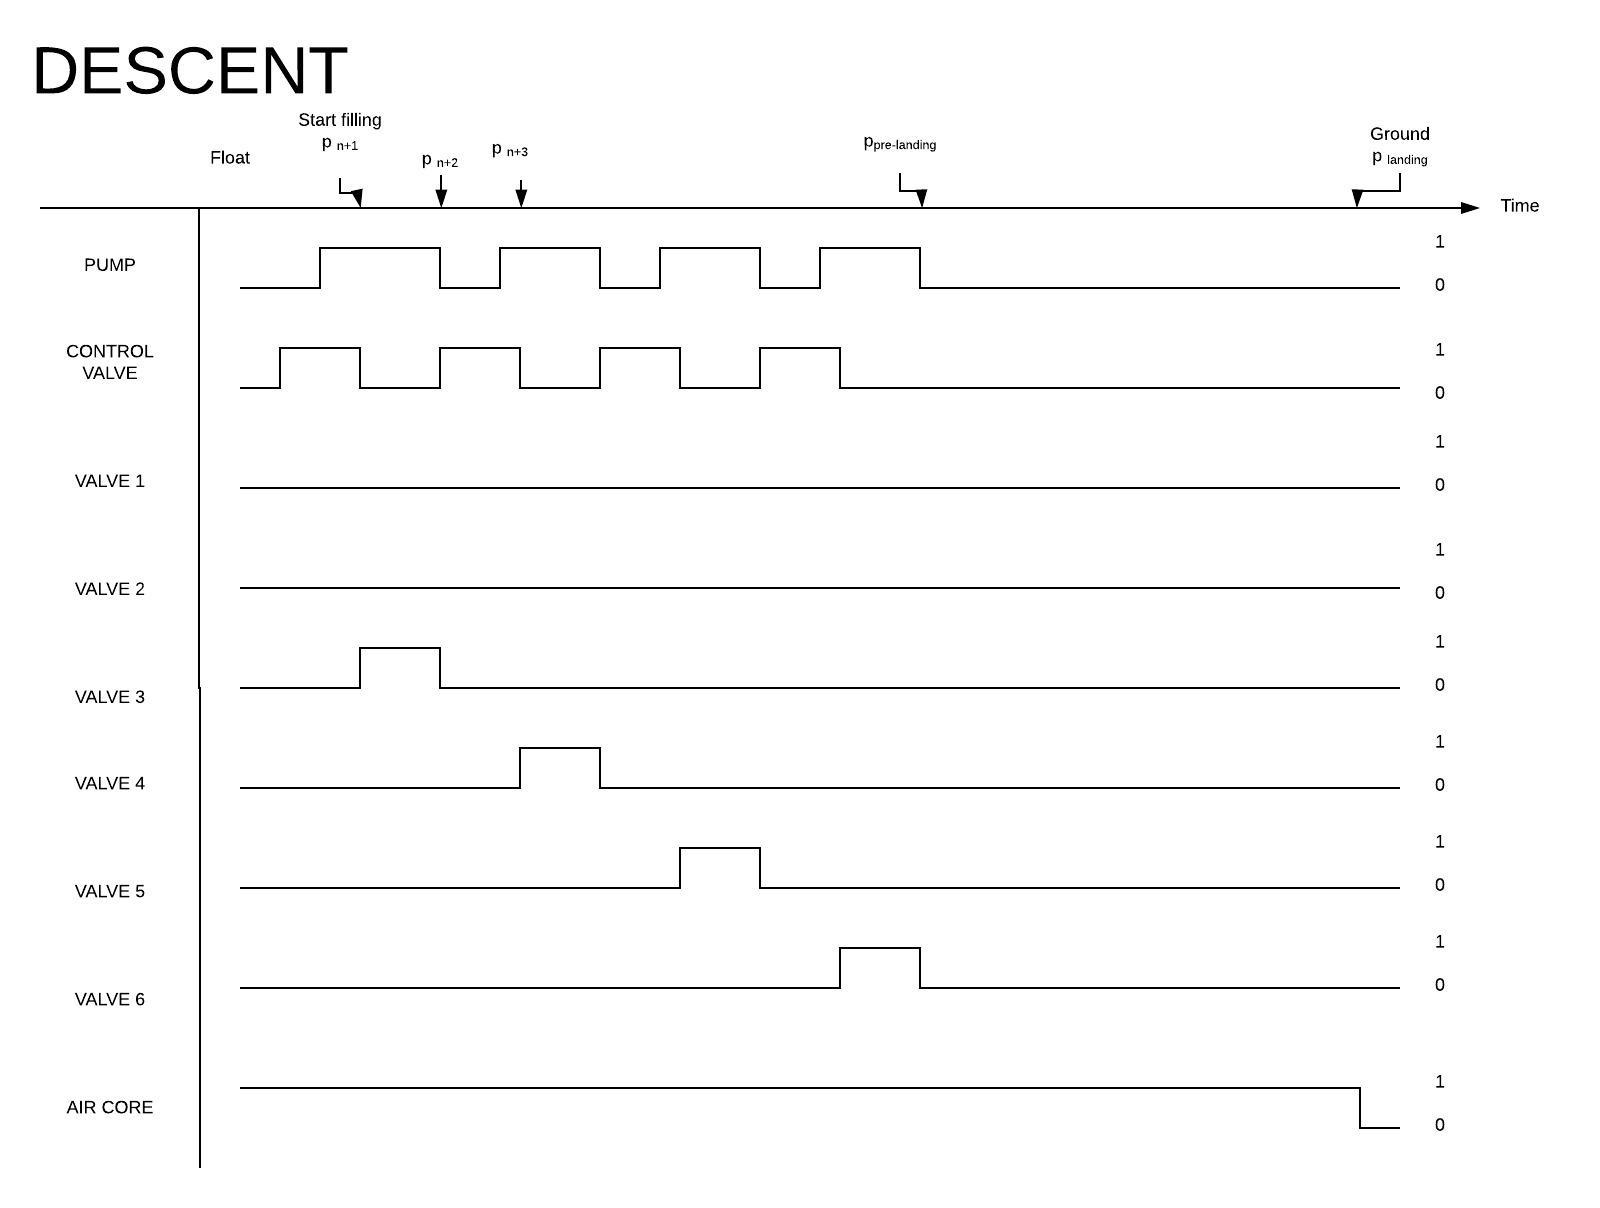
\includegraphics[width=1\linewidth]{4-experiment-design/img/descent-phase.jpeg}
    \end{align*}
    \caption{The Emptying and Sampling Sequence-Descent Phase.\label{fig:descent}}
\end{figure}

In the diagrams, 0 denotes closed/off and 1 denotes opened/on. The horizontal axis denotes the different pressure levels throughout the flight, with p$_0$ being the sea level pressure and p$_8$ being the pressure during Float Phase.

The ambient pressure dependent timeline of the experiment was planned to be as follow:

\textbf{Ascent Phase:}\\
$p_0$ – $p_1$
\begin{itemize}
    \item CAC valve shall be closed.
    \item AAC valves shall be closed.
    \end{itemize}
$p_1$ – $p_2$
\begin{itemize}
    \item CAC valve shall be opened.
    \item CAC tube shall start flushing.
    \end{itemize}
    
$p_2$ – $p_3$
\begin{itemize}
    \item AAC flushing valve shall be opened, allowing for the system to flush.
    \item CAC valve should remain open.
    \end{itemize}
$p_3$ – $p_4$
\begin{itemize}
    \item AAC flushing valve shall be closed.
    \item Valve 1 shall be opened, allowing for air to enter the first bag.
    \item CAC valve should remain open.
    \end{itemize}
$p_4$ – $p_5$
\begin{itemize}
    \item Valve 1 shall be closed.
    \item AAC flushing valve shall be closed.
    \item CAC valve should  remain open.
    \end{itemize}
$p_5$ - $p_6$    
 \begin{itemize}
    \item AAC flushing valve shall be opened, allowing the system to flush. 
    \item CAC valve should remain open.
    \end{itemize}
$p_6$ - $p_7$
\begin{itemize}
    \item AAC flushing valve shall be closed.
    \item Valve 2 shall be opened, allowing for air to enter the second bag.
    \item CAC valve should remain open.
    \end{itemize}
$p_7$ - $p_8$
\begin{itemize}
    \item Valve 2 shall be closed.
    \item AAC flushing valve shall be closed.
    \item CAC shall finish flushing.
    \end{itemize}    
    



\textbf{\\Float Phase:}\\
No action was taken other than continued telemetry.
 
\textbf{Descent Phase:}
 
$p_9$ – $p_{10}$
\begin{itemize}
    \item CAC shall start sampling. 
    \item AAC valves shall be closed.
\end{itemize}

$p_{10}$ – $p_{11}$
\begin{itemize}
    \item AAC flushing valve shall be opened allowing the system to flush.
    \item CAC valve should remain open. 
\end{itemize}
 
  
$p_{11}$ – $p_{12}$
\begin{itemize}
    \item AAC flushing valve shall be closed.
    \item Valve 3 shall be opened, allowing for air to enter the third bag.
    \item CAC valve should remain open. 
\end{itemize}

$p_{12}$ – $p_{13}$
\begin{itemize}
    \item Valve 3 shall be closed.
    \item AAC flushing valve shall be closed.
    \item CAC valve should remain open.
\end{itemize}

$p_{13}$ – $p_{14}$
\begin{itemize}
    \item AAC flushing valve shall be opened allowing the system to flush.
    \item CAC valve should remain open.
\end{itemize}

$p_{14}$ – $p_{15}$
\begin{itemize}
    \item AAC flushing valve shall be closed.
    \item Valve 4 shall be opened, allowing for air to enter the fourth bag.
    \item CAC valve should remain open.
\end{itemize}

$p_{15}$ – $p_{16}$
\begin{itemize}
    \item Valve 4 shall be closed.
    \item AAC flushing valve shall be closed.
    \item CAC valve should remain open.
\end{itemize}

$p_{16}$ – $p_{17}$
\begin{itemize}
    \item AAC flushing valve shall be opened, allowing the system to flush. 
    \item CAC should remain open.
  \end{itemize}

$p_{17}$ – $p_{18}$
\begin{itemize}
    \item AAC flushing valve shall be closed.
    \item Valve 5 shall be opened, allowing for air to enter the fifth bag. 
    \item CAC valve should remain open.
\end{itemize}

$p_{18}$ – $p_{19}$
\begin{itemize}
    \item Valve 5 shall be closed.
    \item AAC flushing valve shall be closed.
    \item CAC valve should remain open.
\end{itemize}

$p_{19}$ – $p_{20}$
\begin{itemize}
     \item AAC flushing valve shall be opened, allowing the system to flush. 
    \item CAC valve should remain open.
   \end{itemize}

$p_{20}$ – $p_{21}$
\begin{itemize}
    \item AAC flushing valve shall be closed.
    \item Valve 6 shall be opened, allowing for air to enter the sixth bag.
    \item CAC valve should remain open.
\end{itemize}

$p_{pre-landing}$ 
\begin{itemize}
    \item Valve 6 shall be closed.
    \item AAC flushing valve shall be closed.
    \item CAC valve shall be opened.
\end{itemize}

$p_{0-landing}$
\begin{itemize}
    \item CAC valve shall be closed.
\end{itemize}


Note: The AAC system's air pump is only on during sampling into the air sampling bags and flushing of the system.


\raggedbottom